\chapter{Object-level vision}
\label{chp:object_level}
\minitoc
\bigskip


The field of computer vision comprises a wide range of methods to extract information about the real world from images taken by digital cameras. 
This information can be used to infer the structure of the environment (mapping or object tracking), about the movement of the system to which is 
attached the camera (localization), or both at the same time (Simultaneous Localization And Mapping, \aka\ SLAM). In the context of robotics, the images 
are obtained one after another at a constant rate. This leads to a somewhat continuous evolution of the image appearance, which can be leveraged in 
various ways  (feature tracking, motion models, etc.). We are here interested in solving SLAM, which is the most general application of this method and 
is used when a robot needs to localize itself in an a priori unknown environment. A vast literature of dedicated algorithms have been developed in this 
regard, with approaches ranging from geometrical constraints using sparse feature detection \cite{mur2015orb, ferrera2021ov} or photometric consistencies 
\cite{newcombe2011dtam, engel2014lsd, engel2017direct}, certain methods combining ideas from both approaches \cite{forster2014svo, forster2016svo}.

These algorithms aim at being generalizable to any kind of environment and have their respective strengths and weaknesses \cite{fuentes2015visual}. 
Although open-source code is available for most, these pieces of software may be difficult to integrate into other frameworks. Besides, 
though providing quite accurate localization, maps obtained from these methods are rarely immediately useful, lacking semantic information about 
the scene. 

In this thesis, rather than investing time and energies in new vision processing algorithms, we chose to focus our attention on legged-robot state estimation. 
In particular, we are interested in localizing the robot with respect to objects of interest such as stairs, tables, or the like, whose geometrical models are known.
Approaches based on object-level measurement can provide an affordable alternative, and are readily available. These systems assume the presence of known objects 
in the scene which can be detected in the images. Dedicated algorithms can then infer the object pose relative to the camera, which can be used to build 
\textit{object-level SLAM} systems. 

In this chapter, we present two measurements models based on available software, that permit the implementation of this paradigm. The first one 
uses unique \apriltag\ fiducial markers \cite{wang2016iros} (to which we may refer to as \textit{tags} informally) that are laid out sparsely in the scene. 
The second uses a deep-learning-based method \cite{labbe2020cosypose}
to obtain relative poses from an object of interest, such as a pair of stairs. Instead of artificially augmenting the environment with fiducial markers, we assume 
that objects of interest exist in the scene, whose CAD models are known. 
Both systems lack ways to estimate the uncertainty of their output and we, therefore, propose methods for the computation of the measurements covariances.

In both models, we assume that we have a calibrated camera and that the images have been corrected for distortions. The camera reference frame $C$ has its origin at 
the camera optical center and follows the convention X-Y-Z = Righ-Down-Front, Front being the optical axis direction, looking through the lens. This chapter starts by 
introducing the measurement model based on a general 6D factor used by both systems. Methods to recover the covariance of both algorithms are then given. 
For applications fusing these models with IMU data, please refer to \chpRef{chp:absolute_vi} and \chpRef{chp:cosyslam}.



\section{Relative 6D pose factor}
In this section, we will derive a general 6D relative transformation factor between a \keyframe\ and a object, whose poses in world frame are respectively $\T{W}{B} \in \SE(3)$ and $\T{W}{O} \in \SE(3)$. In this chapter, we denote by $\T{}{} \in \SE(3)$ 6D transformations.

Let us assume that an algorithm estimates directly $\Tm{C}{O}$, a measurement of the pose of an element 
of the scene with an attached frame $O$ with respect to the camera frame $C$.
The kinematic chain of the problem described in \figRef{fig:camera_object_chain} unrolls as 
$\T{W}{O} = \T{W}{B}\T{B}{C}\T{C}{O}$ where W and B correspond to the world and body frames. $\T{B}{C}$ corresponds to the extrinsic pose 
of the camera.
Given measurement $\Tm{C}{O}$, this relation can therefore be turned into a residual relating 
the robot pose, the camera extrinsics, and the object pose:

\begin{align}
    \bfe_V (\T{W}{B}, \T{B}{C}, \T{W}{O}) 
    &= \left[ (\T{W}{B}\T{B}{C})^{-1}\T{W}{O} \right] \ominus \Tm{C}{O} ~ \in \Reals^6 \\
    &= \Log_{\SE(3)} ( (\T{W}{B} \T{B}{C} \Tm{C}{O})^{-1} \T{W}{O}) ~ \in \Reals^6
\end{align}
%
where here $\Log_{\SE(3)}$ denotes the log map on $\SE(3)$.

Depending on the nature of the problem, we can fix some of the variables of the residual. In table \tabRef{tab:res_var_fix}, various estimation problems are modelled depending on which variable is fixed.

\begin{table}[h]
    \centering
    \begin{tabular}{c|c|c|c}
        & $\T{W}{B}$ & $\T{B}{C}$ & $\T{W}{O}$  \\
        \hline
        \hline
        SLAM with extrinsics calibration &  \checkmark
 &  \checkmark &  \checkmark \\
        \hline
        SLAM &  \checkmark & X &  \checkmark \\
        \hline
        Localization with extrinsics calibration &  \checkmark &  \checkmark & X \\
        \hline
        Localization &   \checkmark & X & X \\
        \hline
        Mapping & X & X &  \checkmark \\
    \end{tabular}
    \caption{Some possible estimation problems corresponding to fixing either of the variables. Estimated variables are checkmarked with " \checkmark
". Fixed variables are marked with "X".}
    \label{tab:res_var_fix}
\end{table}



We also assume that we have access to the covariance of this measurement 
\mbox{$\Cov_V \in \Reals^{6 \times 6}$}. 

This factor is general enough to be used in two applications that we successively describe, based on \apriltag\ fiducial markers and CosyPose. For both, we explain the
the algorithm behind the pose measurements and propose covariance models.

% We will now describe two applications of this factor, one using \apriltag\ fiducial markers and one using 
% a deep-learning object pose estimation algorithm.

\begin{figure}
    \centering
    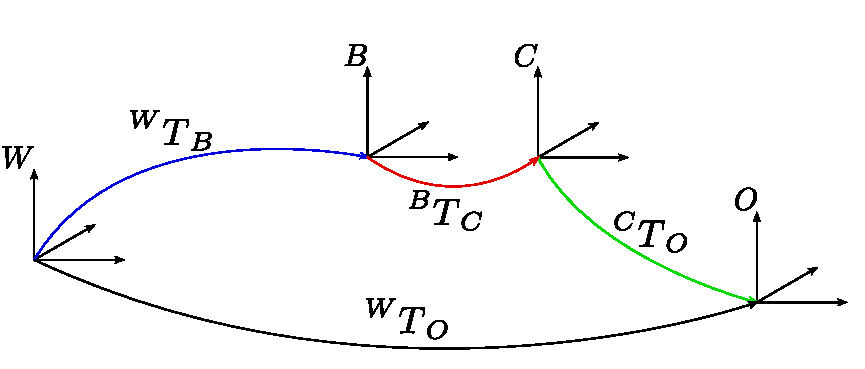
\includegraphics[width=0.7\textwidth]{figures/kin_tree_object.pdf}
    \caption{Kinematic tree of the object/camera measurement model}
    \label{fig:camera_object_chain}
\end{figure}

%
%
\section{Fiducial markers}
\label{sec:fiducial_markers}
\subsection{Markers Pose estimation algorithms}

Fiducial markers (such as ARToolkit \cite{kato1999marker}, ARTag \cite{fiala2005artag}, ArUco \cite{garrido2014automatic}) are widely used in robotics 
and Augmented Reality (AR) applications as they provide an easy way to obtain a relative 6D pose 
between a calibrated camera and the marker. These markers are designed so that they are uniquely and robustly identifiable in any scene 
\cite{wang2016iros,romero2018speeded}. 

The pose extraction happens in two steps. First, the tag corners sub-pixel projections are extracted from the image along with the unique id of the detected tag. 
In this work we used the \apriltag\ library \cite{wang2016iros} for its performances and popularity within the robotics community. Second, knowing the tag size, 
we can compute the position of these corners in the local tag frame, as defined in \figRef{fig:apriltag_coordinate_frame}. Recovering the pose of the tag from the 
corner projections and their local coordinates is then an instance 
of the Perspective-n-Point (PnP) algorithm \cite{gao2003complete}, which requires at least four 2D-3D correspondences to compute a unique solution the 3D pose 
\footnote{The P3P algorithm yields up to four geometrically feasible solutions, a fourth point being then used to select the right one.}. 
A vast literature has been written on the topic, many methods relying on efficient analytical models
\cite{gao2003complete, lepetit2009epnp, collins2014infinitesimal, terzakis2020consistently}, sometimes refined by a nonlinear maximum likelihood step.




\subsection{Ambiguity in the pose estimation}
\label{sec:tag_ambiguity}

A known problem of fiducial markers is the orientation ambiguity of detections in noisy images. This phenomenon may make the PnP estimation of the 
tag orientation jump wildly from one frame to the next. This is due to the fact that the conic perspective projection of the corners is weak, 
that is the difference between two symmetrical tag orientations is very close. If this difference falls below the camera pixel noise, 
then the two solutions are indistinguishable, as shown in \figRef{fig:tag_ambiguity}. This happens especially when the tag corner projection is 
close to a square, that is when the tag is orthogonal to the axis passing through the camera and tag origins. 
We refer to this situation as tags being \textit{fronto-parallel} with respect to the camera.
This phenomenon is intensified when the tag is far from the camera as it spans a smaller region of the image. 

\begin{figure}
    \centering
    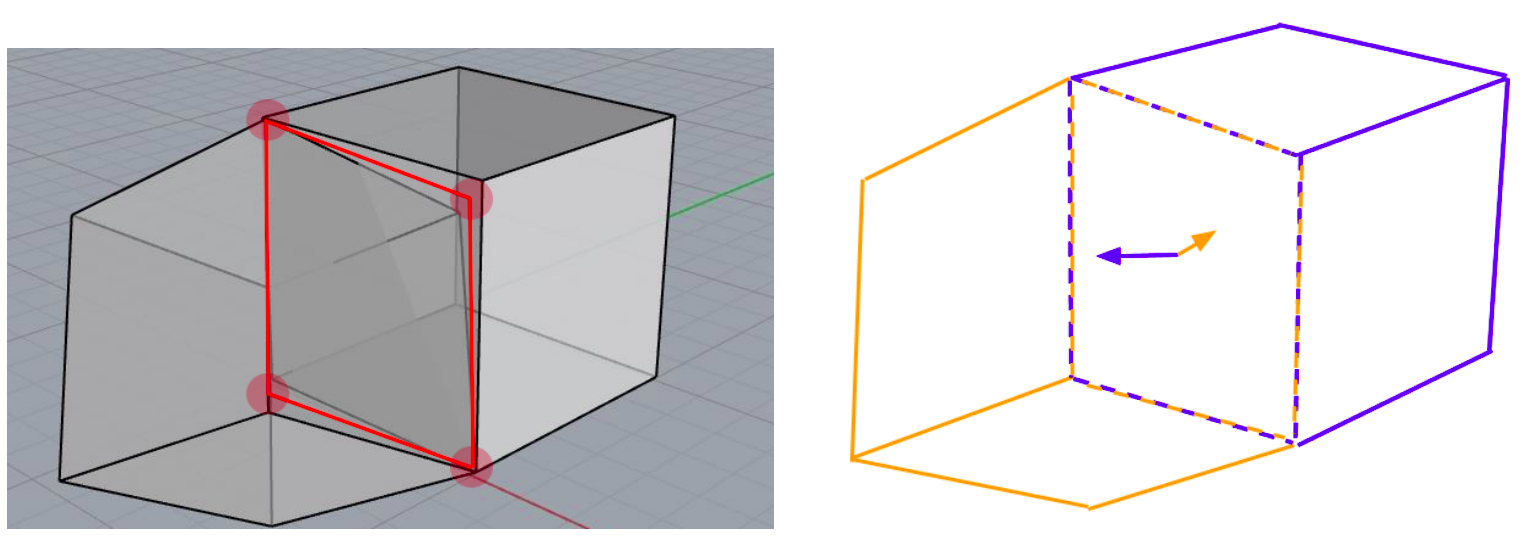
\includegraphics[width=0.7\textwidth]{figures/tag_ambiguity.png}
    \caption{Illustration of the tag ambiguity problem. The red circles represent uncertainty in the corner detection due to pixel noise. 
    The conic perspective projections of faces from two cubes with 120 degrees orientation difference fall withing these regions and are, therefore, 
    hard to distinguish. Figure taken from \cite{8206468}.}
    \label{fig:tag_ambiguity}
\end{figure}

One solution is to define the tag factor residual as the pixel error between the detected corners and their projection given the
current tag pose estimate and let the optimizer find the most probable tag poses given the complete set of measurements. However, if one tag is wrongly initialized, 
the optimizer is not guaranteed to leave the local minimum with new measurements. 

Our solution is to bring the disambiguation to the front-end side.
\cite{collins2014infinitesimal} provides an implementation of the PnP problem that retrieves both ambiguous poses. When expressed in the camera frame, 
both solutions share the tag position and differ only in their orientation. We typically want to select the solution with the smallest error. 
However, if the reprojection errors $e_1$ and $e_2$ are too close (we test for $\tfrac{e_2}{e_1} < h$ with $e_1 \leq e_2$ and $h$ an empirical threshold), 
we increase the rotational part of the covariance matrix by a great factor to cancel the influence of the wrong tag orientation on the 
overall MAP problem

\subsection{Covariance model}
\label{sec:apritlag_covariance}
Obtaining a covariance of the estimated transformation is an important step toward the integration of these measurements in a sensor fusion algorithm.

Urban \cite{urban2016mlpnp} (Eq. (23)) uses a careful parameterization of the homogeneous coordinates associated with 2D features to develop
a maximum likelihood PnP algorithm and also proposes a covariance model based on the problem Hessian (Eq. (23)).  However, the particular choice of variable 
parameterization makes the formulation of the covariance computation overcomplicated.
We think that a simpler yet equivalent formulation is possible. 

Usually, when a nonlinear mapping of noise variables from one space to another is available, we can propagate the covariance through the nonlinearity
as shown in Eq. \eqRef{eq:cov_propagation}. 
Instead of directly obtaining Jacobians from the PnP algorithms, we found that a natural way to proceed is to take the opposite 
direction as follows. It should somehow be possible, knowing the marker size and the relative pose measurement, and assuming pixel noise, to
recover $\Cov_{\T{}{}}$. A simple model of pixel noise is to assume isotropic Gaussian noise on the pixels. If we stack four pixel (the four tag corners) 
$\bfx_i = [u_i, v_i] \in \Reals^2$ in the column vector $\bfx = [\bfx_1~\bfx_2~\bfx_3~\bfx_4]\tr$, we have therefore that
$\bfx$ is corrupted by a Gaussian noise $\Cov_{\bfx} = \sigma_{x}^2 \bfI_8$, where $\sigma_{x}$ usually takes values of 1 or 2 pixels.
The PnP algorithm provides us with a function $\text{pnp}$ defined as:

\begin{equation}
    \begin{split}
        \text{pnp}_w: \Reals^8 &\rightarrow \SE(3) \\
                           \bfx &\rightarrow \T{C}{O} = \text{pnp}_w(\bfx)
    \end{split}
\end{equation}
%
where w denotes the dependency on the width of the marker. This $\text{pnp}_w$ function implementation depends on the specificities of the PnP algorithm used and  
is in general hard to analytically differentiate. Instead, if we consider the inverse function.

\begin{equation}
    \begin{split}
        \text{proj}_w: \SE(3) &\rightarrow \Reals^8 \\
                           \T{C}{O} &\rightarrow \bfx = \text{proj}_w(\T{C}{O})
    \end{split},
\end{equation}

This function $\text{proj}$ maps the relative pose to the projection of the tag in the image, a rather simple Jacobian expression can be derived using the chain rule, as follows.

We denote the marker corner coordinates in the marker frame as shown in \figRef{fig:apriltag_coordinate_frame}. As a convention 
\cite{wang2016iros}, we order the corners counter-clockwise starting from bottom-left (looking straight at the tag). 

\begin{equation}
    \bfc =
    \begin{pmatrix}
    \bfc_1 \\ \bfc_2 \\ \bfc_3 \\ \bfc_4
    \end{pmatrix}
    ~~
    \bfc_1 =  \begin{pmatrix} -\frac{w}{2} \\ \frac{w}{2} \\ 0 \end{pmatrix}
    ~ 
    \bfc_2 =  \begin{pmatrix} \frac{w}{2} \\ \frac{w}{2} \\ 0 \end{pmatrix}
    ~
    \bfc_3 =  \begin{pmatrix} \frac{w}{2} \\ -\frac{w}{2} \\ 0 \end{pmatrix}
    ~
    \bfc_4 =  \begin{pmatrix} -\frac{w}{2} \\ -\frac{w}{2} \\ 0 \end{pmatrix}.
\end{equation}

%
\begin{figure}
    \centering
    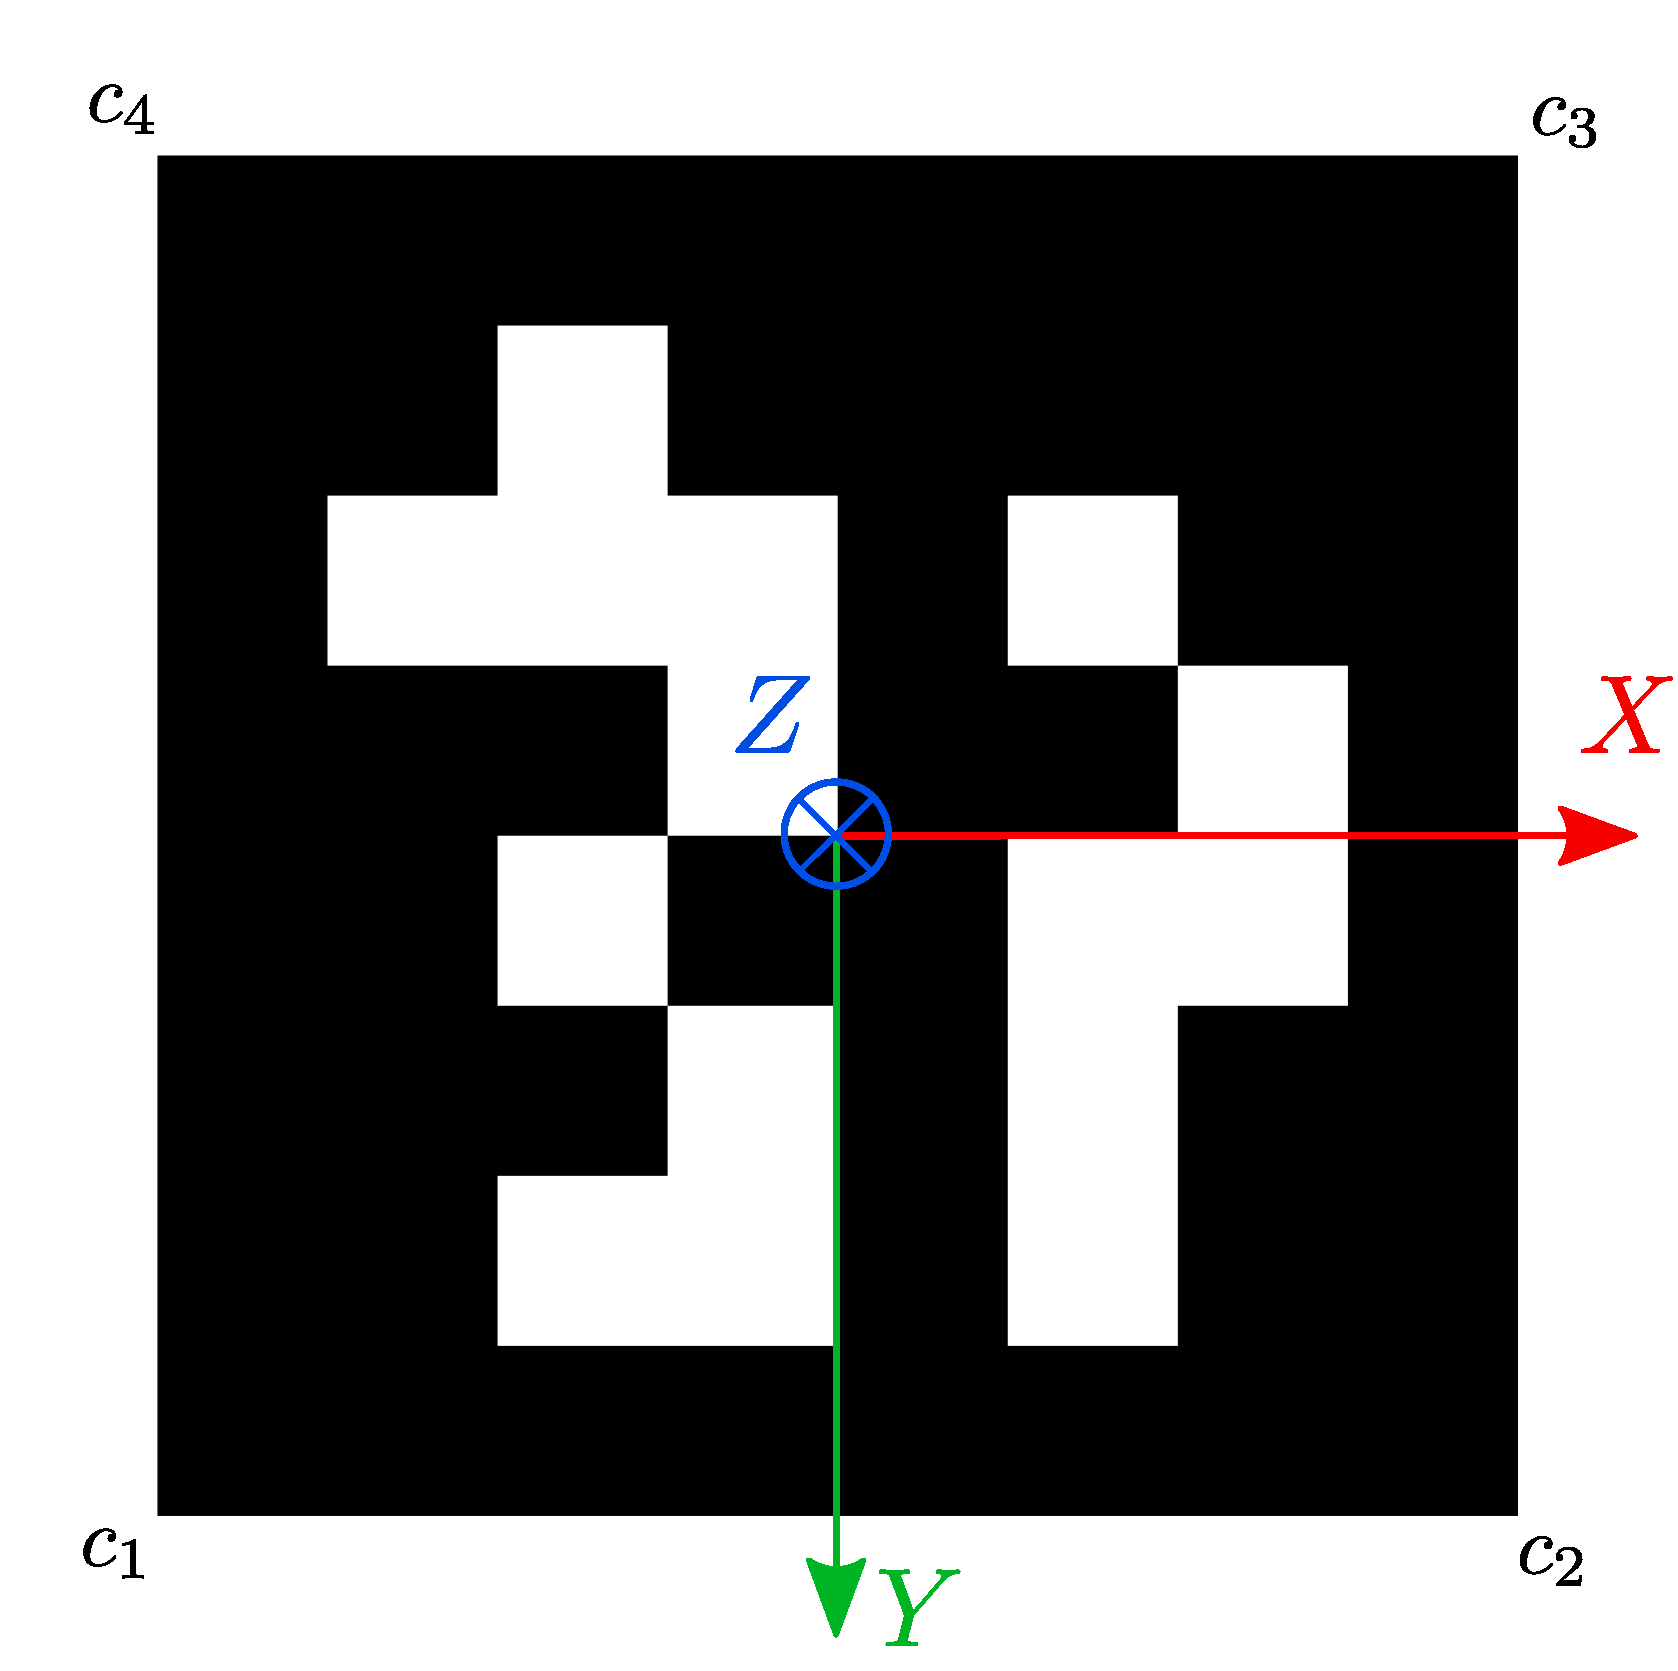
\includegraphics[width=0.5\textwidth]{figures/tag12_frame.png}
    \caption{\apriltag~local coordinate systems and corners conventions \cite{wang2016iros}}
    \label{fig:apriltag_coordinate_frame}
\end{figure}

Then, assuming that images are corrected (no distortion), the pinhole camera model gives us that

\begin{equation}
    \bfx_i = \text{eucl}(\bfh_i) = \text{eucl}(\bfK\T{C}{O} \bfc_i)
\end{equation}
%
for each corner $c_i$, where $h_i$ are the homogeneous coordinates representing the projected corners and $eucl$ is the function that maps 
homogeneous coordinates to euclidean pixel coordinates defined as
%
\begin{equation}
    \begin{split}
        \text{eucl}: \Reals^3 
        &\rightarrow \Reals^2 \\
        \bfh = \begin{pmatrix}x\\y\\z\end{pmatrix} 
        &\rightarrow \bfx = \begin{pmatrix}x/z\\y/z\end{pmatrix}
    \end{split}.
\end{equation}

We need to compute the Jacobian of each corner projection with respect to the estimated relative pose, decomposed using the chain rule as  

\begin{equation}
    \bfJ^{\bfx_i}_{\T{}{}} = \bfJ^{\bfx_i}_{\bfh_i} \bfJ^{\bfh_i}_{\T{}{}}.   
\end{equation}

Regarding the transformation, we will consider it to be an element of the composite Lie group $\left<\Reals(3)\times \SO(3)\right>$ since the translation and rotation part 
of transformation are treated separately in our solver. The expressions of those functions are, therefore, expressed as:

\begin{equation}
    \begin{split}
        &\bfh_i = \bfK(\Rot{C}{O}\bfc_i + \posi{C}{O}) \\
        &\bfJ^{\bfh_i}_{\posi{C}{O}} = \bfK ~~~~~~ \\ &\bfJ^{\bfh_i}_{\Rot{C}{O}} = -\bfK\Rot{C}{O}[\bfc_i]_{\times}  \\  
        &\bfJ^{\bfh_i}_{\T{C}{O}} = [\bfJ^{\bfh_i}_{\posi{C}{O}} ~~~ \bfJ^{\bfh_i}_{\Rot{C}{O}}] = \bfK [\bfI_3 ~~~ -\Rot{C}{O} [\bfc_i]_{\times}]
    \end{split}
\end{equation}
%
while the Jacobian of the map from homogeneous coordinates to euclidean pixels is
\begin{equation}
    \bfJ^{\bfx_i}_{\bfh_i}
    =
    \begin{pmatrix}
    1/z_i & 0 & -x_i/z_i^2 \\
    0 & 1/z_i & -y_i/z_i^2
    \end{pmatrix}.
\end{equation}

Finally, we stack the 4 Jacobians to get the full Jacobian to be used for covariance propagation:
%
\begin{equation}
    \bfJ \triangleq \bfJ^{\bfx}_{\T{C}{O}}=
    \begin{pmatrix}
    \bfJ^{\bfx_1}_{\T{C}{O}} \\ 
    \bfJ^{\bfx_2}_{\T{C}{O}} \\ 
    \bfJ^{\bfx_3}_{\T{C}{O}} \\ 
    \bfJ^{\bfx_4}_{\T{C}{O}}
    \end{pmatrix}
    ~ \in \Reals^{8 \times 6}
\end{equation}.

We therefore have the covariance propagation equation $\Cov_{\bfx} = \bfJ \Cov_{\T{}{}} \bfJ\tr$. 
This equation must be inverted in order to recover the needed covariance $\Cov_{\T{}{}}$. $\bfJ$ being non square and full column rank for four 
corners ($\bfJ \in \Reals^{8 \times 6}$, we can use the right pseudo inverse $\bfJ^{+} = (\bfJ\tr \bfJ)^{-1}\bfJ\tr$. Multiplying left and right by 
respectively $\bfJ^{+}$ and $\bfJ^{+,\top}$, we obtain: $\Cov_{\T{}{}} = \bfJ^{+} \Cov_{\bfx} \bfJ^{+,\top}$. Given that the pixel noise covariance is 
isotropic as explained above, $\Cov_{\bfx} = \sigma_x^2 \bfI$, this equation finally simplifies to:

\begin{align}
    \Cov_{\T{}{}} 
    &=  (\bfJ\tr \bfJ)^{-1}\bfJ \tr \sigma_x^2 \bfI ((\bfJ\tr \bfJ)^{-1}\bfJ\tr)\tr \\
    &=  \sigma_x^2 (\bfJ\tr \bfJ)^{-1} \bfJ\tr \bfJ (\bfJ\tr \bfJ)^{-1} \\
    &= \sigma_{x}^2(\bfJ\tr \bfJ)^{-1}.
\end{align}

Note that the derivations above are not limited to a square tag with four corners and could be used for any object defined as
a set of points in its local coordinate system provided their configuration is not degenerate and makes the PnP computation possible \cite{gao2003complete}.  
We have therefore a compact model informed by the geometry of the measurement model with a single tuning parameter in the pixel noise $\sigma_x$.


\subsection{Covariance visualization}

It is hard to represent graphically the appearance of this uncertainty model from the full 6D covariance. However, we can inspect the positional and 
orientational uncertainty (respectively the 3x3 upper-left and 3x3 lower-right sub-matrices) by representing them as confidence ellipsoids.

The principle is the following. For a 3D random variable $x \sim \Gaussian{\mu}{\Cov}$ described by a multivariate normal 
distributions with mean ${\bf\mu} \in \Reals^3$ and 
covariance matrix $\Cov \in \Reals^{3 \times 3}$, the statistics:
%
\begin{equation}
    (\bfx - {\bf\mu})\tr \Cov^{-1}(\bfx - {\bf\mu}) = \chi^2
    \label{eq:chi2}
\end{equation}
%
follows a chi-square distribution with 3 degrees of freedom. Since \eqRef{eq:chi2} is the equation of an ellipse centered at $\mu$ and shape 
governed by $\Cov$, we can then plot confidence volumes as ellipsoids by replacing the right-hand side of  
\eqRef{eq:chi2} by the critical value of the chi-square distribution for the desired confidence interval (we chose $\alpha=99\%$). 

We simulate a realistic scenario using calibration data from a laboratory RealSense camera, 15cm tags and $\sigma_x = 2~\text{pixels}$. 
\figRef{fig:apriltag_cov_P} and \figRef{fig:apriltag_cov_P} show how the uncertainty on position and orientation relate to different factors.

\begin{figure}[h]
    \centering
    \begin{subfigure}{.50\linewidth}
        \centering
        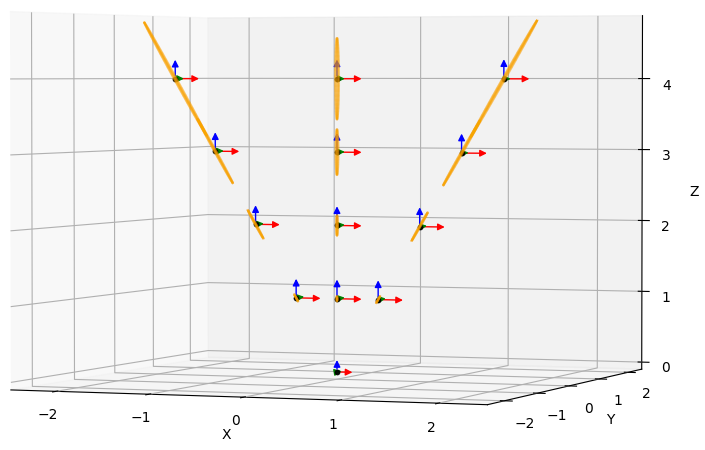
\includegraphics[width=\textwidth]{figures/apriltag_cov_P_015.png}
        \caption{Relative position covariances, 15cm tags \label{fig:apriltag_cov_P_015}}
    \end{subfigure}%
    \hfill
    \begin{subfigure}{.50\linewidth}
        \centering
        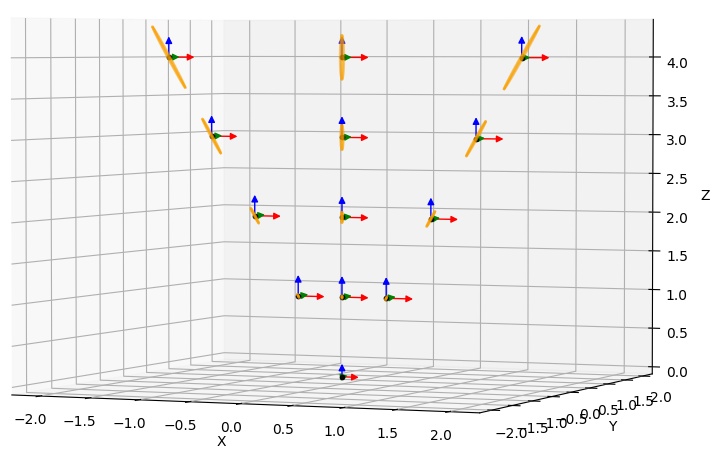
\includegraphics[width=\textwidth]{figures/apriltag_cov_P_030.png}
        \caption{Relative position covariances, 30cm tags \label{fig:apriltag_cov_P_030}}
    \end{subfigure}%
    \caption{Position uncertainty from the analytical covariance model. The single frame at the bottom represents the pose of the virtual camera, others are identical 
    \apriltags placed in front of the camera at different distances but identical orientations. Covariances are represented in orange, centered at the corresponding tag 
    position.
    (\subref{fig:apriltag_cov_P_015}) shows that the main positional uncertainty is along the camera-tag axis, which corresponds to the distance information. 
    In (\subref{fig:apriltag_cov_P_030}), tags are twice the size, which shrinks their position uncertainty.}
    \label{fig:apriltag_cov_P}
\end{figure}

In all cases, the covariance increases with the distance to the camera (the volume of the ellipses increases).
On top of that, we can see that, for both position and orientation, the uncertainty distribution is clearly anisotropic: 
the uncertainty of the pose measurements is logically higher in the dimensions that lead to the least change in the aspect of the tag projection. 

For the position uncertainty (\figRef{fig:apriltag_cov_P}), the shape of the covariance is easily interpretable: the uncertainty is the highest along the camera-tag axis.
Besides, this uncertainty is not much influenced by the relative camera-tag orientation. 

For the orientation uncertainty (\figRef{fig:apriltag_cov_O}), the shape of the covariance is harder to interpret: a high uncertainty about the orientation along 
one axis corresponds to a dilatation of the ellipse along this axis. For instance, in \figRef{fig:apriltag_cov_O_10deg}, tags placed
along the Z-axis of the camera frame have a very high uncertainty along the X and Y-axis (in camera frame). Their uncertainty ellipses seem, therefore, very flat
along the Z-axis. \figRef{fig:apriltag_cov_O_10deg} directly relates to our discussion about tag pose ambiguity in \secRef{sec:tag_ambiguity}. Tags close
to fronto-parallel configuration (along the camera Z-axis) have a very high rotational uncertainty compared to tags that have a more important relative 
orientation as in \figRef{fig:apriltag_cov_O_10deg}.


\begin{figure}[h]
    \centering
    \begin{subfigure}{.50\linewidth}
        \centering
        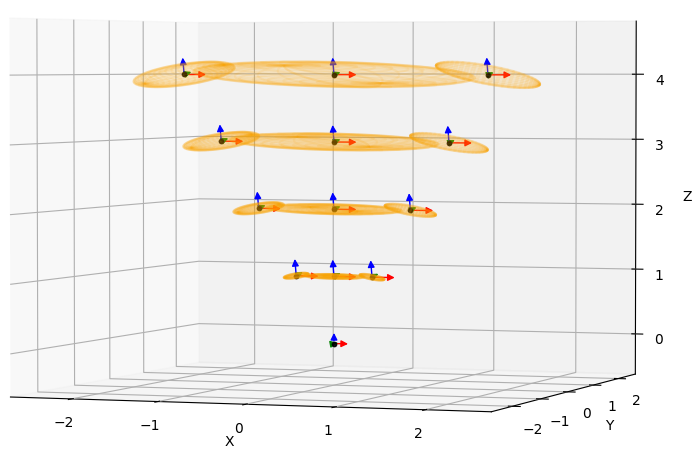
\includegraphics[width=\textwidth]{figures/apriltag_cov_O_10deg.png}
        \caption{Relative orientation covariances, 10 degree orientation \label{fig:apriltag_cov_O_10deg}}
    \end{subfigure}%
    \hfill
    \begin{subfigure}{.50\linewidth}
        \centering
        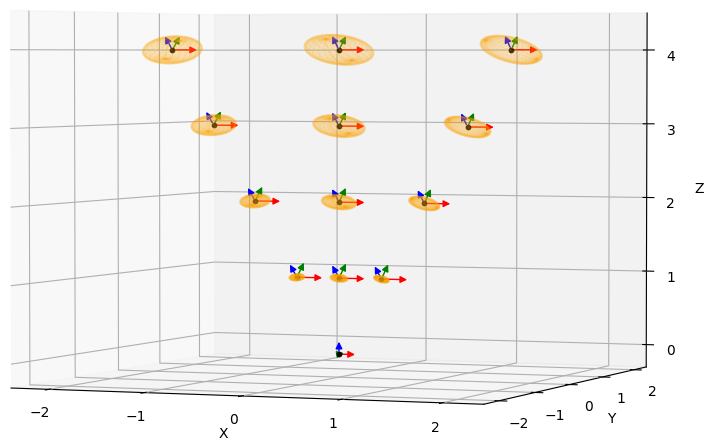
\includegraphics[width=\textwidth]{figures/apriltag_cov_O_45deg.png}
        \caption{Relative position covariances, 45 degree orientation \label{fig:apriltag_cov_O_45deg}}
    \end{subfigure}%
    \caption{Orientation uncertainty from the analytical covariance model. The single frame at the bottom represents the pose of the virtual camera, others are identical 
    \apriltags placed in front of the camera at different distances but identical orientations. Covariances are represented in orange, centered at the corresponding tag 
    position.
    In (\subref{fig:apriltag_cov_O_10deg}) . 
    (\subref{fig:apriltag_cov_O_45deg}) shows the same configuration for tag twice the size, whose relative position is less uncertain.}
    \label{fig:apriltag_cov_O}
\end{figure}


In \figRef{fig:apriltag_proj}, 3 tags are projected: the first (black) is half a meter away from the camera in fronto-parallel orientation, the second (orange)
10cm to the right, and the third (rose) 10cm behind. We can see that the appearance of difference of appearance due to a depth-wise movement is much smaller, which 
explains the higher uncertainty on the depth measurement.

\begin{figure}[h]
    \centering
    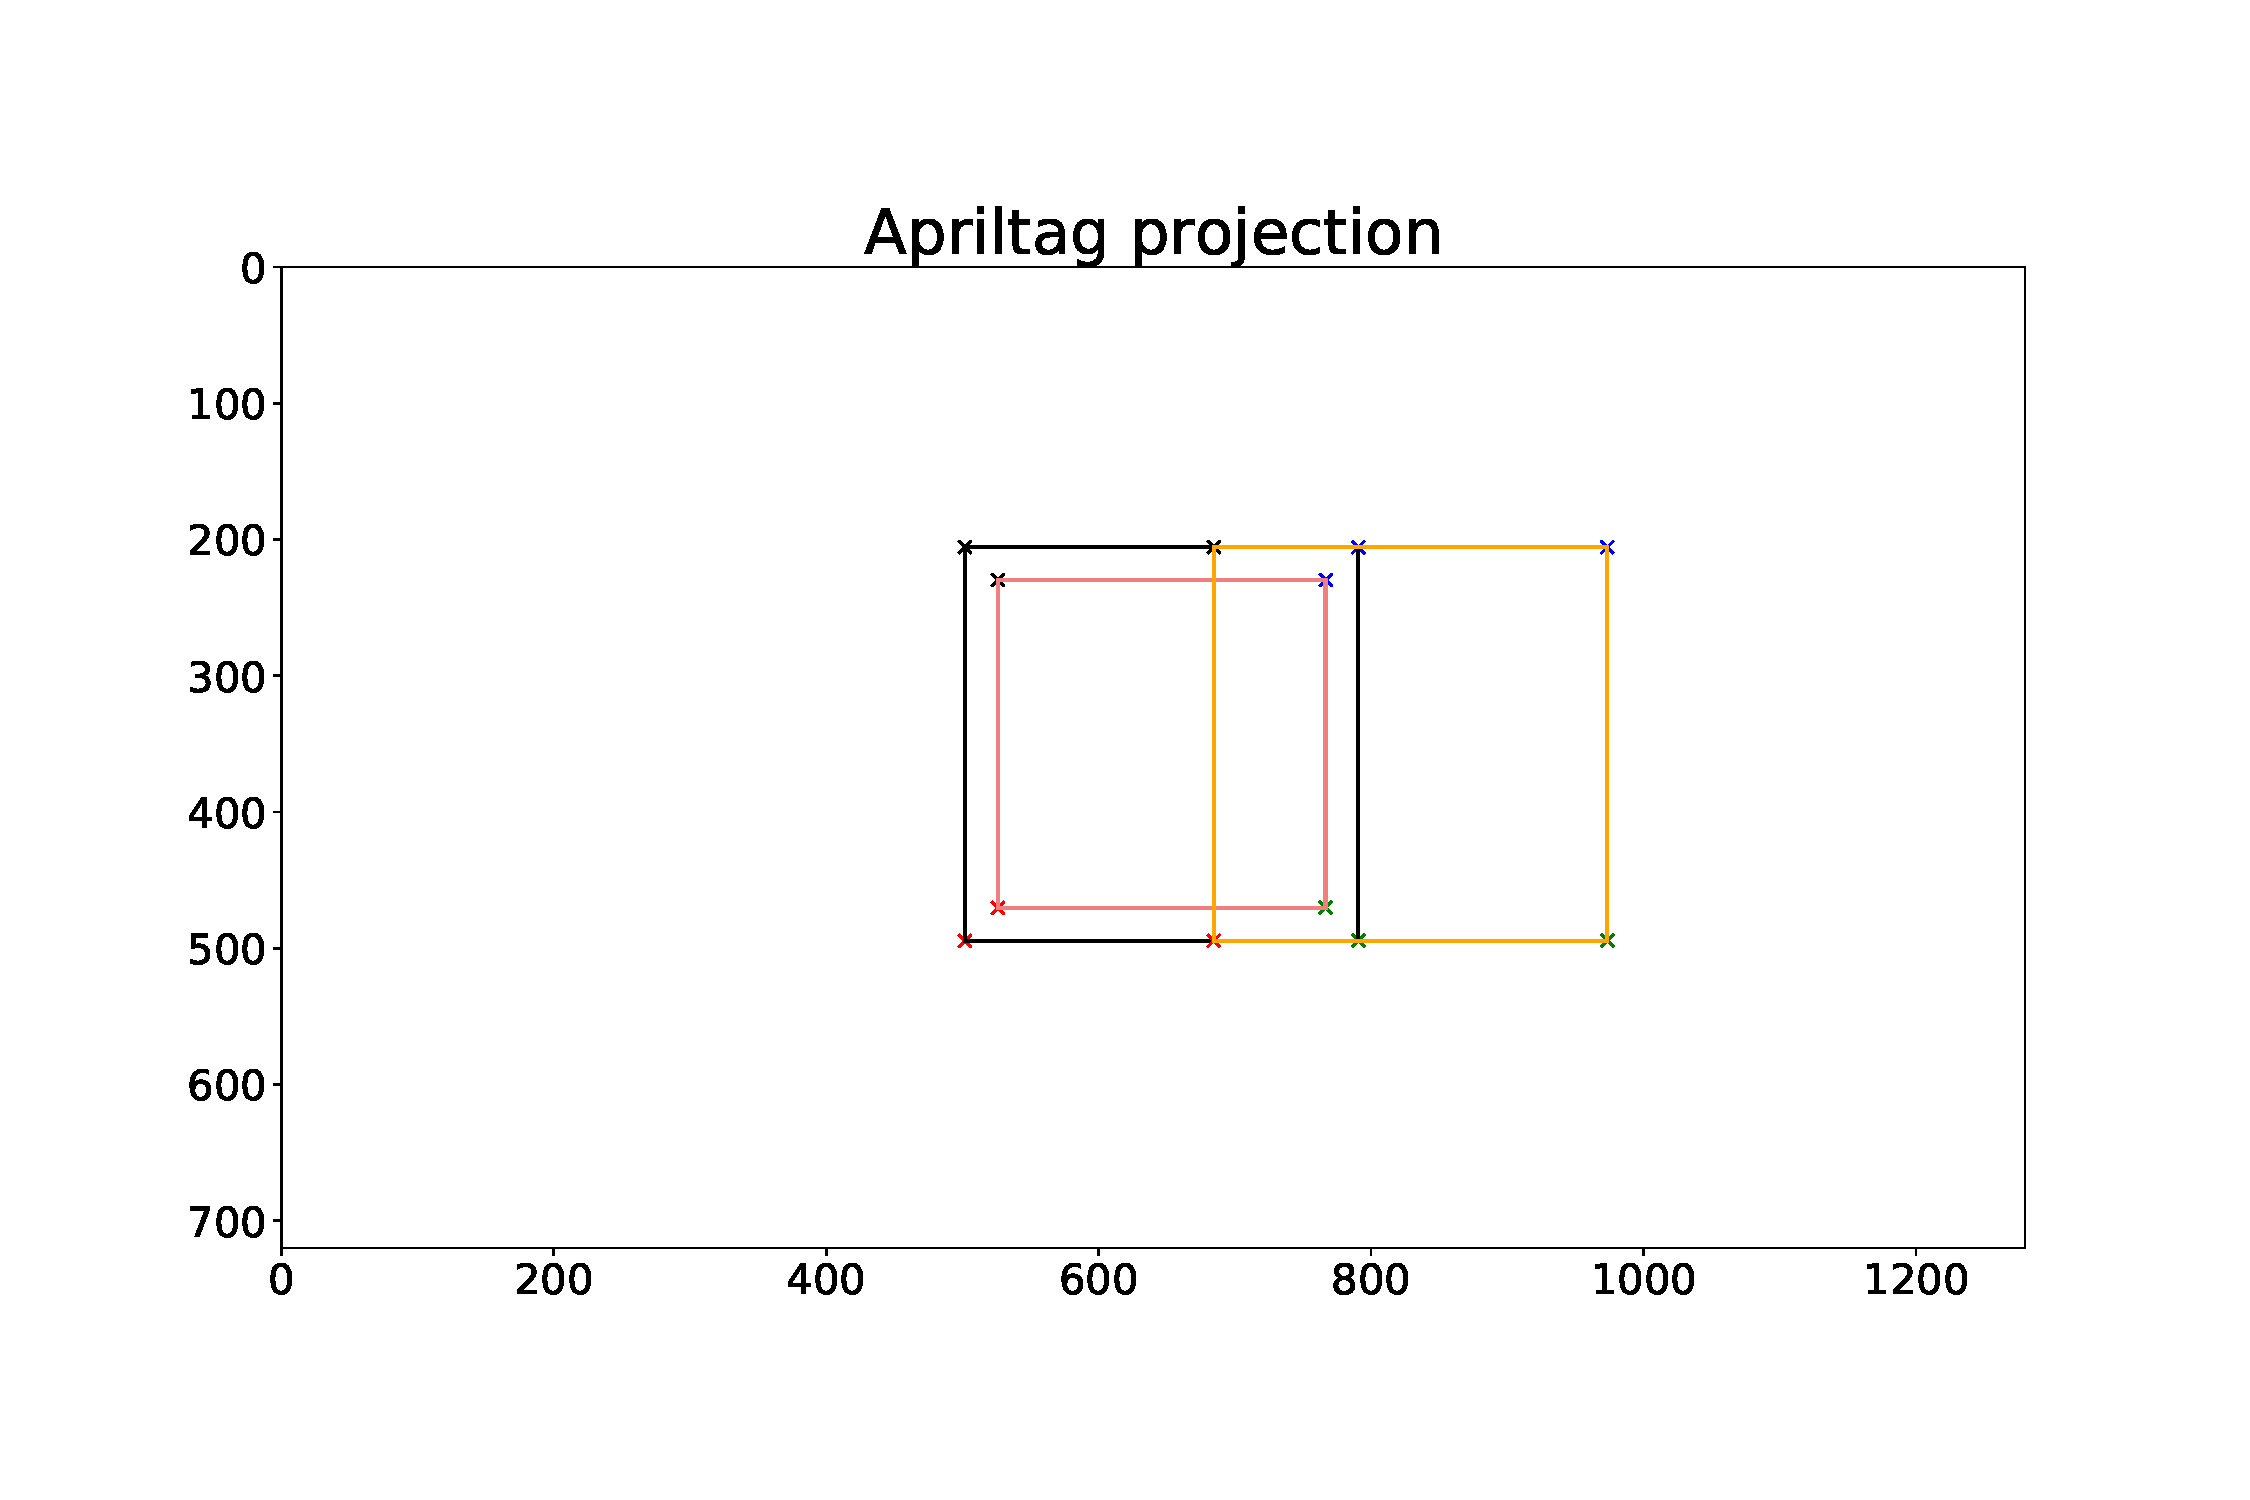
\includegraphics[width=0.8\textwidth]{figures/apriltag_proj.pdf}
    \caption{Projection of 3 tags of camera frame position: black -> (0,0,0.5), orange -> (0.1,0,0.5), rose -> (0.0,0,0.6)}
    \label{fig:apriltag_proj}
\end{figure}

This covariance seems well behaved and captures the physical intuitions about the measurement uncertainties. 
This was leveraged in the context of a visual-inertial SLAM system implemented in \chpRef{chp:absolute_vi}. 
A quantitative comparison with \cite{urban2016mlpnp} would be interesting as well as an experimental validation campaign to further strengthen our results.


%
%
%
%
\section{Learning-based object pose estimation}
\label{sec:learning_based_object_pose_est}
In this section, we propose to integrate a deep-learning-based algorithm to object pose estimation \cite{labbe2020cosypose} to our measurement models. 


\subsection{Object pose estimation}
\label{sec:object_pose_est_algos}
The problem of object pose estimation can simply be stated: given a calibrated camera and a set of known object models, detect those objects in the current image 
frame and extract camera-objects poses. Traditionally, competing methods were developed using either local features matching or learning-based methods.
As shown by the most recent BOP challenge results \cite{hodan2020bop}, deep-learning methods now clearly dominate the field in terms of accuracy. 
At the time of the writing, the highest-ranking non-learning based pose extraction method \cite{konig2020hybrid} (object detection is deep learning based) 
actually uses depth measurement measurements and is dominated by a purely RGB, deep-learning-based model \cite{haugaard2021surfemb}, though \cite{konig2020hybrid} 
seems to be ten times faster \footnote{BOP challenge leaderboard is available at \url{https://bop.felk.cvut.cz/leaderboards/}}.

In terms of accuracy, these results advocate for the use of deep-learning purely RGB image-based methods, that now provide accurate enough results 
for these to be used in robotics applications \cite{labbe2021single}. 
We use the CosyPose model of Labbe et al. \cite{labbe2020cosypose} which at the time ranked first in the BOP challenge leaderboard.
This approach mixes a new state-of-the-art single-view pose estimation algorithm with a multi-view algorithm using RANSAC and Bundle Adjustment. 
This system obtains precision in the order of centimeters 
on real objects whose 3D model is known. Its performances make it a good candidate as a direct 6D pose sensor to perform a multi-sensor fusion. 
In the context of legged robots, this is very useful to localize the robot relative to objects it needs to interact with, such as objects 
to manipulate or stairs to climb. While CosyPose is not yet able to generalize to unseen classes of objects, rapid progress is expected in 
this direction.

\subsection{CosyPose}
The front end of the SLAM system designed for this project includes object detection and object pose estimation. 
This function is provided by CosyPose \cite{labbe2020cosypose}, a deep-learning-based 6D pose estimator that reaches state-of-the-art
 performances for 6D object pose estimation.
In the original paper, a single-view pose estimator and a multi-view algorithm were introduced. In our context, only the single-view module is used, 
while object tracking is handled by the SLAM framework. 

CosyPose takes as input a single image $I$ and a set of 3D models, each associated with an object label $l$. The camera $C$ is assumed to be calibrated. 
A set of object detections is performed using the object detector Mask-RCNN \cite{he2018mask}. Each 2D candidate detection is identified 
by an index $\alpha$ and associated with an object candidate $O_{\alpha}$. Its 6D pose $\T{C}{O_{\alpha}} \in \SE (3)$ relative to the camera $C$ 
is then computed as follows.

\begin{figure}[]
    \begin{subfigure}{.5\textwidth}
        \centering
        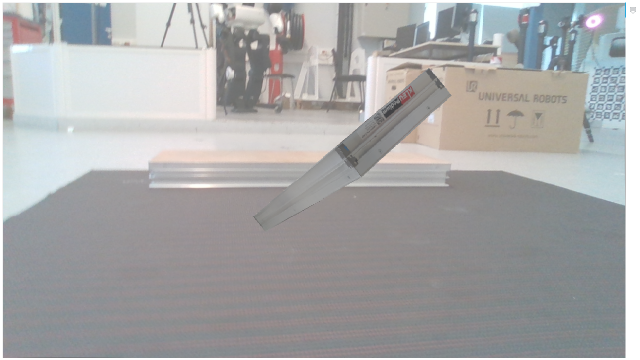
\includegraphics[width=.9\linewidth]{figures/cosyslam/convergence_1.png}  
    \end{subfigure}
    \begin{subfigure}{.5\textwidth}
        \centering
        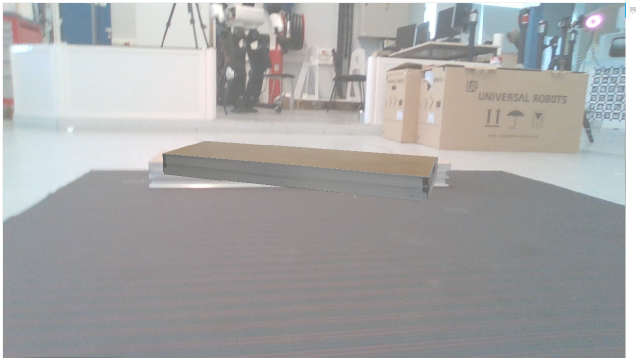
\includegraphics[width=.9\linewidth]{figures/cosyslam/convergence_2.png}  
    \end{subfigure}

    \label{fig:fig}
    \begin{subfigure}{\textwidth}
        \centering
        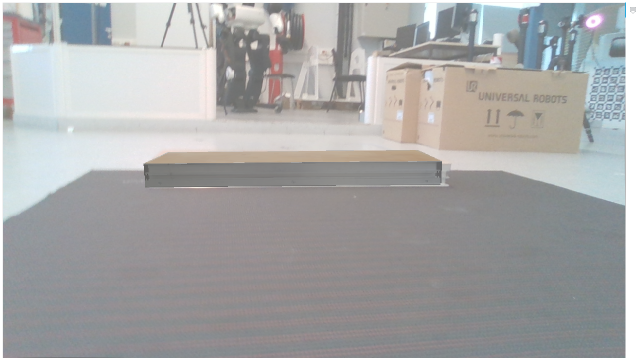
\includegraphics[width=.45\linewidth]{figures/cosyslam/convergence_3.png}
    \end{subfigure}
    \caption{Progressive convergence of a stair step estimated pose over successive iterations of CosyPose.}
    \label{fig:cosypose-convergence}
\end{figure}


The single-view procedure for pose estimation of CosyPose is an improvement over the one proposed in DeepIm \cite{deepim_2019}. The general idea is to iteratively 
use the same neural network to iteratively converge to the object pose (\figRef{fig:cosypose-convergence}). It takes as input the cropped image of the detected 
object bounding box and a rendered image based on the current object pose solution $\T{C}{O_{\alpha},k-1}$ at iteration $k-1$. 
It returns a transformation update $\T{O_{\alpha},k-1}{O_{\alpha},k}$ that brings the rendered image closer to the cropped image. In practice, 
two neural networks with the same structure are trained independently: one for coarse pose estimation, \ie, the first iteration of the iterative process, 
and another for the refinement of the pose. The coarse network gives the first transformation $\T{C}{O_{\alpha},0}$, 
and the prediction of the pose of the object is obtained by composing the $N$ successive transformations:

\begin{equation}
\T{C}{O_{\alpha}} = \T{C}{O_{\alpha},0} \prod_{k=1}^N  \T{O_{\alpha},k-1}{O_{\alpha},k}.
\end{equation}

CosyPose reuses the neural network architecture of DeepIm with a new backbone for feature extraction, Efficient-Net \cite{tan2020efficientnet} ,
with a spatial average pooling layer added after it. Then, it disables the optical flow sub-network during the training. 
A new rotation parametrization, introduced in \cite{zhou2020continuity}, is used for the loss function, which has been shown 
to bring more stability during training. Then, the focal length of the cropped images is recomputed during training to fit the virtual camera 
of these images. Finally, the object symmetries are taken into account during training thanks to the \textit{symmetric distance}. 
Each 3D model $l$ is associated with a set of symmetries $S(l)$, that is the set of transformations that leave the aspect of the object unchanged:

\begin{equation}
    \textit{S}(l) = \left \{ \bfS \in \SE(3) | \forall \bfT \in \SE(3), \cR(l,\bfT) = \cR(l,\bfT \bfS)\right \}
\end{equation}
%
where $\cR(l,\bfT)$ is the rendered image of the object $l$ captured in pose $M$. Given a set of symmetries $S(l)$, 
the symmetric distance $D_l$ measures the distance between two 6D poses represented by transformation $\bfT_1$ and $\bfT_2$. 
Given an object $l$ associated to a set $\cX_l$ of 3D points $\mathbf{x} \in \cX_l$, we have:

\begin{equation}
    D_l(\bfT_1, \bfT_2) = \underset{\bfS \in \textit{S}(l)}{\text{min}} \frac{1}{|\cX_l|} \sum_{\mathbf{x} \in \cX_l} ||\bfT_1 \bfS \mathbf{x} - \bfT_2\mathbf{x} ||^2.
    \label{eq:distSym}
\end{equation}

Equation \eqRef{eq:distSym} measures the average distance between the points of the object model transformed by $\bfT_1$ and $\bfT_2$ according to the symmetry 
that best aligns the transformed points. In practice, for continuous symmetries  that are rotations around an axis (like for instance for a textureless cylinder), 
$S(l)$ is discretized using 64 angles.


\subsection{Empirical covariance estimation}
\label{sec:cosypose_covariance}

When considering merging a tracker such as CosyPose with other sensor modalities, an important aspect is to predict covariance representing the level 
of confidence in the tracker estimate. Such data uncertainty is crucial to the robustness of SLAM systems involving neural networks 
subsystems such as \cite{yang2020d3vo}. The depth-based object SLAM algorithm \cite{SalasMoreno2013SLAMSL} claimed to compute a covariance matrix approximated 
as the inverse of the Iterative Closest Point output. The methods targeted for deep learning applications are harder to implement, especially if the goal 
is to use an off-the-shelf pose estimation neural network, as is the case for this paper. For instance, Bayesian Neural Networks \cite{jospin2020hands} 
need to be trained explicitly for uncertainty prediction while Monte Carlo (MC) Dropout \cite{gal2016dropout} requires multiple forward passes at run-time.

In our work CosySLAM \cite{debeunne2021cosyslam}, we present a practical implementation of a SLAM system based on the design of an off-the-shelf deep learning object 
pose estimation algorithm \cite{labbe2020cosypose}, which empirical results are presented in \chpRef{chp:cosyslam}. 
To integrate these measurements with other sensors, we propose a noise model based on empirical data.

\subsubsection{Covariance model}

CosyPose does not provide an evaluation of its uncertainty.
%
The two main families of solutions available to estimate uncertainties of neural network predictions consist in MC dropout \cite{gal2016dropout} 
or Bayesian Neural Network (BNN) \cite{jospin2020hands}. Using BNNs would require changing the architecture of CosyPose and retraining it. 
MC dropout would require several forward passes through the network for each iteration, which would be computationally expensive. 

We need to compute the covariance without changing the architecture of the network and at an affordable cost. 
We propose to make an empirical error model based on polynomial regression in order to compute the covariance matrix. 
The idea is to parametrize the average error on each $\se(3)$ component returned by CosyPose. We conducted an empirical study on several video 
sequences that explore the variations of the parameter set for several object types. The error is computed by comparing the $\SE(3)$ transformations 
between the camera $C$ and an object $O$ returned by CosyPose $\T{C}{O}$ with the same transformation given by a motion capture system. 
We then use the error predictions of our parametric model as a proxy to the true 6 covariances during model fitting. 
A different model is fit for each object type due to their diversity of shapes, sizes, and textures.

The parameters used to compute the error need to represent the error sources of CosyPose as much as possible. 
To cover the error due to the configuration of the object in space, we need to include the 3D coordinates of the camera in the object frame. 
We also want to take into account some invariance that can occur by rotating around the object if it is texture-less for example. 
For this reason, we choose spherical coordinates of the camera origin with respect to the object frame to parametrize the model. 
Another source of error can be the occlusion of the object in the scene, as well as the motion blur, or any inherent noise in the image. 
This can affect the quality of the detection and of the pose estimation. Mask-RCNN returns a confidence score $s$ for each detection 
that we will include in our model. This score is the output of the final softmax layer of the detector and can be interpreted
as the level of confidence Mask-RCNN has in its prediction.

% To sum up, we have the following parameters for our error model:
% \begin{itemize}
% \item $\displaystyle r = || \posihat{O}{C}||$,
% \item $\displaystyle \varphi  = \arctan\left(\frac{ \prescript{0}{}{\hat{x}}_C}{\prescript{0}{}{\hat{y}}_C}\right)$,
% \item $\displaystyle \theta  = \arcsin\left(\frac{\prescript{0}{}{\hat{z}}_C}{r}\right)$,
% \item $\displaystyle s$ : mask-RCNN softmax output.
% \end{itemize}

To sum up, our model is parameterized by four values: $r$ - distance, $\varphi$ - azimuth, $\theta$ - elevation, $s$ - Mask-RCNN softmax output. 


\begin{figure}
    \centering
    \begin{subfigure}{0.47\textwidth}
        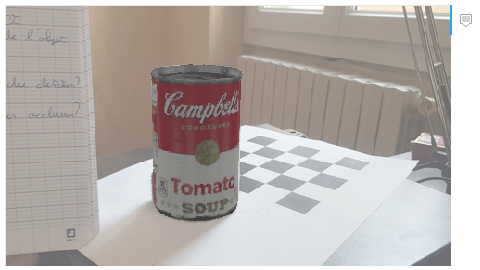
\includegraphics[width=\textwidth]{figures/cosyslam/s999.png}
        \caption{$s$~=~0.999}
    \end{subfigure}
    \begin{subfigure}{0.47\textwidth}
        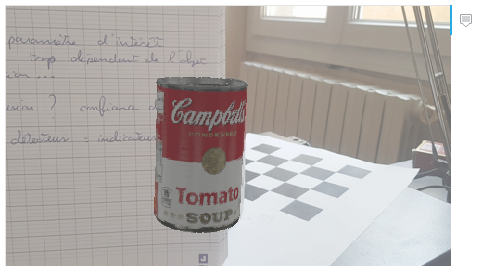
\includegraphics[width=\textwidth]{figures/cosyslam/s996.png}
        \caption{$s$~=~0.996}
    \end{subfigure}
    \caption{Example of values of the Mask-RCNN softmax output for various levels of occlusion. 
    These shows the impressive robustness of the CosyPose to partial occlusions.}
\end{figure}

We can then compute the error of CosyPose relative to the motion capture data: 

\begin{equation}
    \mathbf{e}  = [\mathbf{e}_{t}, \mathbf{e}_{a}]  \triangleq  \left[~\posihat{O}{C} - \posim{O}{C}, ~ \Log \left(\Rothat{O}{C}^{-1}\Rotm{O}{C}\right)~\right]
\end{equation}
%
where $\widehat{\cdot}$ and $\widetilde{\cdot}$ denote quantities obtained from the motion capture system and CosyPose respectively. 
$\Log$ denotes the logarithm application mapping elements of SO(3) to the $\Reals^3$ representation of its Lie algebra 
$\so(3)$.

We want to find a polynomial function $f(r, \varphi, \theta, s) \in \mathbb{R}^6$ that returns the error given the set of training data $\{X,E\}$. 
For each object, we capture a set of video sequences and we compute the error with the motion capture data for each measurement. 
We then perform polynomial regression with a pipeline in Scikit Learn \cite{scikit-learn}. A simple linear regression leads to a high root-mean-square error (RMSE) 
on a test dataset. Over degree 3, the model overfits and the high curvature of the polynomial returned high error values outside of the training data range. 
Thus, a degree 2 polynomial regression seemed to offer a good compromise.  Quantitative results are given in the experimental validation section 
(see Fig.~\figRef{fig:empirical_err} for a few examples of fitted polynomials).


In general, this empirical model led to good experimental results, with the drawback that it needs to be trained (ideally with real data)
for each new object. If possible, the covariance model should directly result from CosyPose nominal training.
We started to investigate this direction (with the Msc thesis of Cesar Debeunne) but mostly let it be here as an open perspective.




\subsubsection{Empirical covariance}

As explained in Sec. II, we have trained empirical models to evaluate the covariance of the estimation of CosyPose. 
To validate these models, we propose to exhibit a few intuitive observations and quantitative statistical analysis. 
One of the parameters involved in our model is the absolute distance between the camera and the object, noted $r$. 
Our trained models show an expected behavior regarding this parameter: the global error increases when the camera moves away from the object. 
%
\begin{figure}[h]
  \centering 
  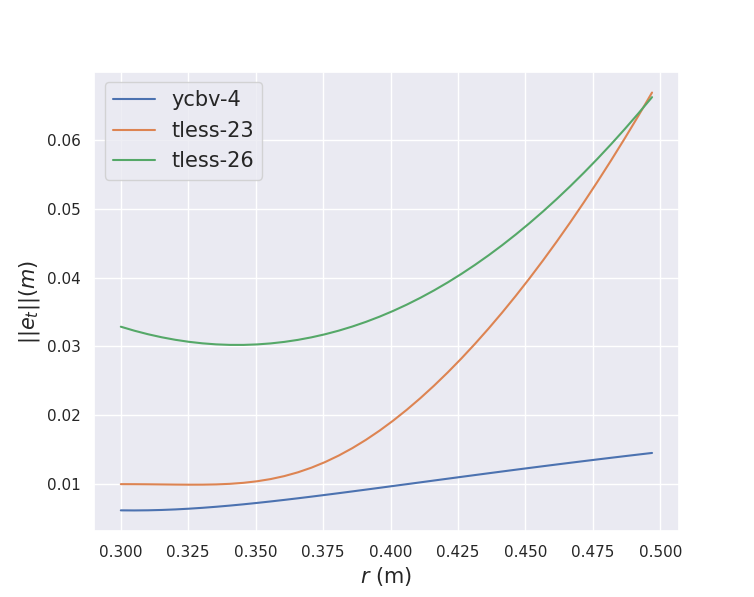
\includegraphics[width=0.8\textwidth]{figures/cosyslam/empirical_err.png}
  \caption{The norm of the translation error returned by the models of three different objects with respect to $r$, the distance between the camera and the object. 
            The other parameters $\theta$, $\phi$ and $s$ are fixed to the average values of our training data. }
  \label{fig:empirical_err}
\end{figure}

\figRef{fig:empirical_err} sheds light on these phenomena and gives an explicit comparison between the models of different objects. 
The error of the object from the YCBV dataset seems more stable and smaller than the one of the objects from the T-LESS dataset. 
This can be explained by the texture of the object and the absence of symmetries: T-LESS objects are known to be more challenging 
for pose estimation and this is confirmed by our model.

A more quantitative evaluation can be deduced from table \tabRef{tab:empirical_models}. The translation error seems to be captured pretty well,
 as the RMSE is around the centimeter. However, the angular error seems a little less predictable, especially for T-LESS objects whose orientation 
 estimation can suffer from an important measurement noise due to the lack of textures. The $R^2\in[0,1]$ score is the coefficient of determination 
 and is often used to evaluate statistical models. Its interpretation is subject to debate and cannot conclude by itself on the absolute quality of the model. 
 However, a score higher than 0 demonstrates that the model is more accurate than a baseline average model.

\begin{table}[h]
    \centering
    \caption{A quantitative evaluation of our models, these values are computed on test samples that were not used for training. }
    \begin{tabular}{|c|c|c|c|}
        \hline 
          & $\displaystyle R^{2}$ & RMSE ang. err. (°) & RMSE trans. err. (cm) \\
        \hline 
         YCBV-4 & 0.55 & 5,1 & 0.6 \\
        \hline 
         T-LESS-23 & 0.5 & 11.7 & 1.5 \\
        \hline 
         T-LESS-26 & 0.68 & 22 & 0.6 \\
         \hline
    \end{tabular}
    \label{tab:empirical_models}
\end{table}



\subsection{Retraining with stairs}
\label{sec:retraining_with_stairs}
In order to produce a realistic SLAM scenario in the context of legged robots, we retrained CosyPose with staircases present in our lab.
We made a textured mesh of a stair step used in our experimental platform. This textured mesh was used both for training and using the trained model. 
The generation of photorealistic synthetic data was handled by BlenderProc \cite{denninger2019blenderproc}. The render-and-compare loop uses PyBullet \cite{coumans2021}.

\begin{figure}[h]
    \centering
    \begin{subfigure}[]{{.33\linewidth}}
        \centering
        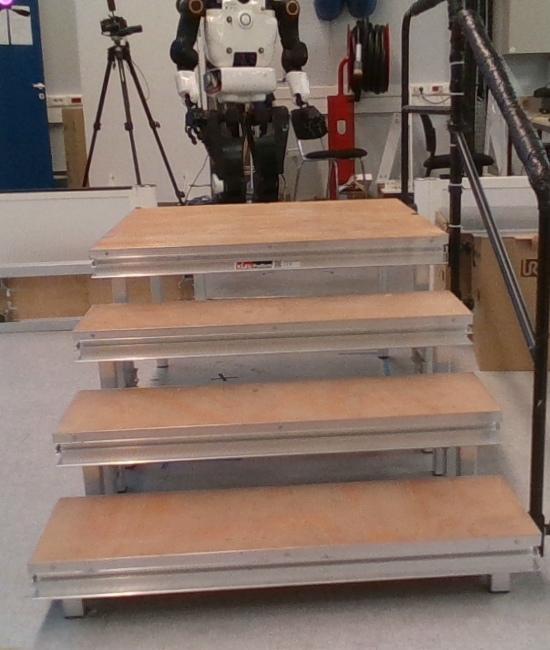
\includegraphics[width=\textwidth]{figures/cosyslam/0006.png} 
    \end{subfigure}
    \hspace{2cm}
    \begin{subfigure}[]{{.33\linewidth}}
        \centering
        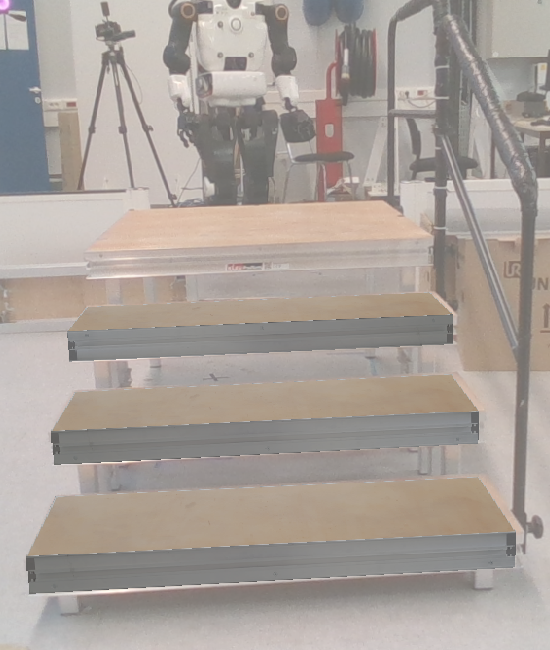
\includegraphics[width=\textwidth]{figures/cosyslam/0006_proj.png} 
    \end{subfigure}
    \caption{On the left, a picture of our climbing module at LAAS and on the right the 3D model of the stair projected according to CosyPose measurements on the same picture}%
    \label{fig:cosypose-ycbv}%
\end{figure}

We generate 10.000 synthetic images that are labeled with object pose ground truths. We retrain the three modalities of CosyPose: 
the Mask-RCNN detector, the coarse pose estimator, and the pose refiner. We slightly tune the training parameters used for the object from the BOP challenge as 
the scale is different: the stair is $1m \times 0.3m \times 0.07m$ whereas a T-LESS object is never wider than $10cm$. 
Thus, we generate training data on $10m \times 10m$ scenes, and we increase the noise used to train the refiner.  

An illustration of the performances of CosyPose on a set of 3 stair steps is given on \figRef{fig:cosypose-ycbv}: 
the pose of each step is here independently estimated which leads to local accuracy but global inconsistency. 



\section{Conclusion}

In this chapter, we have introduced our 2 first practical factors. Both
handle a direct relation between the camera and an object of the scene,
hence being related to semantic (or object-level) SLAM.
The first factor, using fiducial markers, mostly has a practical interest and
will be used in the first experimental setup to validate the IMU factors.
It mostly boiled down to defining a new uncertainty model, that we were able to
analytically derive directly from the PnP algorithm.
The singularity of the 4 point projections are simply handled by rejecting rotation
information when it is detected.
The same factor is then extended to handle a complete object pose estimator,
that we have implemented on top of the award-winning CosyPose detector.
Here also we have tried to directly derivate the uncertainty model from the
algorithm (by training a neural network able to predict both the mean and
the covariance), but finally relied on an empirical model trained a posteriori.
Beyond the practical interest of this new perception feature inserted in the
MAP framework, this second work also contributed to the domain of
neural-based object pose estimation, by proposing a sound and generic
way of sequential estimation, i.e. aggregating measurements across time and
fusing them with other sensors (IMU, etc) to improve the estimation quality.
We will experimentally show in the last part of this thesis the importance
of this temporal sensor fusion, as CosyPose alone, despite the quality of the
algorithm, is not able to provide enough performance guarantee to be
embedded in a robot feedback loop.

This chapter paves the way to extending our work to true semantic SLAM,
i.e mapping while directly extracting the location of an object of interest. With
CosyPose, we directly identify the accurate pose of known objects. This is
important in our context for two reasons. First, the recognized objects can
later be used to close the localization loop with a high degree of accuracy.
Second, the object can be used (\eg in a motion planner) even if out of the
perception range of the robot. A direct practical use case is for the legged
robot to step on an object that is typically not in the field of view (because
legged robots typically do not have cameras pointing on their feet).
While the inclusion on the MAP framework seems satisfactory in practice,
some interesting theoretical work might focus on the insertion of raw
information extracted from the trackers, instead of the overall object pose.
This would avoid possible singularities to invalidate the complete pose
information while partial information might benefit the MAP estimator
(as we already discussed in the practical case of the PnP algorithm for
fiducial markers), or even including latent information directly in the MAP.
It is also important to work on a more systematic way of evaluating the
uncertainty, in particular for neural-based estimators. Finally, some recent
work on extending object pose estimator to classes of objects, or even to
unseen objects, open very interesting directions to extend this work
to semantic SLAM.
